\documentclass[noauthor,nooutcomes,handout,hints,12pt]{ximera}
\graphicspath{  
{./}
{./whoAreYou/}
{./drawingWithTheTurtle/}
{./bisectionMethod/}
{./circles/}
{./anglesAndRightTriangles/}
{./lawOfSines/}
{./lawOfCosines/}
{./plotter/}
{./staircases/}
{./pitch/}
{./qualityControl/}
{./symmetry/}
{./nGonBlock/}
}


%% page layout
\usepackage[cm,headings]{fullpage}
\raggedright
\setlength\headheight{13.6pt}


%% fonts
\usepackage{euler}

\usepackage{FiraMono}
\renewcommand\familydefault{\ttdefault} 
\usepackage[defaultmathsizes]{mathastext}
\usepackage[htt]{hyphenat}

\usepackage[T1]{fontenc}
\usepackage[scaled=1]{FiraSans}

%\usepackage{wedn}
\usepackage{pbsi} %% Answer font


\usepackage{cancel} %% strike through in pitch/pitch.tex


%% \usepackage{ulem} %% 
%% \renewcommand{\ULthickness}{2pt}% changes underline thickness

\tikzset{>=stealth}

\usepackage{adjustbox}

\setcounter{titlenumber}{-1}

%% journal style
\makeatletter
\newcommand\journalstyle{%
  \def\activitystyle{activity-chapter}
  \def\maketitle{%
    \addtocounter{titlenumber}{1}%
                {\flushleft\small\sffamily\bfseries\@pretitle\par\vspace{-1.5em}}%
                {\flushleft\LARGE\sffamily\bfseries\thetitlenumber\hspace{1em}\@title \par }%
                {\vskip .6em\noindent\textit\theabstract\setcounter{question}{0}\setcounter{sectiontitlenumber}{0}}%
                    \par\vspace{2em}
                    \phantomsection\addcontentsline{toc}{section}{\thetitlenumber\hspace{1em}\textbf{\@title}}%
                     }}
\makeatother



%% thm like environments
\let\question\relax
\let\endquestion\relax

\newtheoremstyle{QuestionStyle}{\topsep}{\topsep}%%% space between body and thm
		{}                      %%% Thm body font
		{}                              %%% Indent amount (empty = no indent)
		{\bfseries}            %%% Thm head font
		{)}                              %%% Punctuation after thm head
		{ }                           %%% Space after thm head
		{\thmnumber{#2}\thmnote{ \bfseries(#3)}}%%% Thm head spec
\theoremstyle{QuestionStyle}
\newtheorem{question}{}



\let\freeResponse\relax
\let\endfreeResponse\relax

%% \newtheoremstyle{ResponseStyle}{\topsep}{\topsep}%%% space between body and thm
%% 		{\wedn\bfseries}                      %%% Thm body font
%% 		{}                              %%% Indent amount (empty = no indent)
%% 		{\wedn\bfseries}            %%% Thm head font
%% 		{}                              %%% Punctuation after thm head
%% 		{3ex}                           %%% Space after thm head
%% 		{\underline{\underline{\thmname{#1}}}}%%% Thm head spec
%% \theoremstyle{ResponseStyle}

\usepackage[tikz]{mdframed}
\mdfdefinestyle{ResponseStyle}{leftmargin=1cm,linecolor=black,roundcorner=5pt,
, font=\bsifamily,}%font=\wedn\bfseries\upshape,}


\ifhandout
\NewEnviron{freeResponse}{}
\else
%\newtheorem{freeResponse}{Response:}
\newenvironment{freeResponse}{\begin{mdframed}[style=ResponseStyle]}{\end{mdframed}}
\fi



%% attempting to automate outcomes.

%% \newwrite\outcomefile
%%   \immediate\openout\outcomefile=\jobname.oc
%% \renewcommand{\outcome}[1]{\edef\theoutcomes{\theoutcomes #1~}%
%% \immediate\write\outcomefile{\unexpanded{\outcome}{#1}}}

%% \newcommand{\outcomelist}{\begin{itemize}\theoutcomes\end{itemize}}

%% \NewEnviron{listOutcomes}{\small\sffamily
%% After answering the following questions, students should be able to:
%% \begin{itemize}
%% \BODY
%% \end{itemize}
%% }
\usepackage[tikz]{mdframed}
\mdfdefinestyle{OutcomeStyle}{leftmargin=2cm,rightmargin=2cm,linecolor=black,roundcorner=5pt,
, font=\small\sffamily,}%font=\wedn\bfseries\upshape,}
\newenvironment{listOutcomes}{\begin{mdframed}[style=OutcomeStyle]After answering the following questions, students should be able to:\begin{itemize}}{\end{itemize}\end{mdframed}}



%% my commands

\newcommand{\snap}{{\bfseries\itshape\textsf{Snap!}}}
\newcommand{\flavor}{\link[\snap]{https://snap.berkeley.edu/}}
\newcommand{\mooculus}{\textsf{\textbf{MOOC}\textnormal{\textsf{ULUS}}}}


\usepackage{tkz-euclide}
\tikzstyle geometryDiagrams=[rounded corners=.5pt,ultra thick,color=black]
\colorlet{penColor}{black} % Color of a curve in a plot



\ifhandout\newcommand{\mynewpage}{\newpage}\else\newcommand{\mynewpage}{}\fi


\title{The pinwheel tiling}
\author{Bart Snapp}

\begin{document}
\begin{abstract}
   We are going to investigate a very special triangle that we can use
   to make the \textit{pinwheel tiling}.
\end{abstract}
\maketitle

\begin{listOutcomes}
\item Think about scaling and its relationship to perimeter and area.
\item Think about aperiodic tilings.
\item Tell others about aperiodic tilings.
\item Understand the construction of the pinwheel tiling.
\end{listOutcomes}

Now we learn of the \textit{pinwheel tiling}. While this tiling is
aperiodic and uses only one shape, it is \textbf{not an einstein}
tiling, since there are many ways to make periodic tilings with
triangles.


\mynewpage

\begin{question}
The pinwheel tiling is based on the following triangle:
\[
\includegraphics[width=.3\textwidth]{pinwheelBase.pdf}
\]

\begin{enumerate}
\item If the shortest side of the shaded triangle has a length of 1
  unit, compute the perimeter and area of the shaded triangle
  above. How does this relate to the perimeter and area of the larger
  triangle?

\vfill
  
\item To ``inflate'' the pinwheel triangle, we view the larger
  triangle as being the shaded triangle in our base triangle, then
  draw the other four triangles accordingly. Inflate the triangle
  below two times.
  \[
  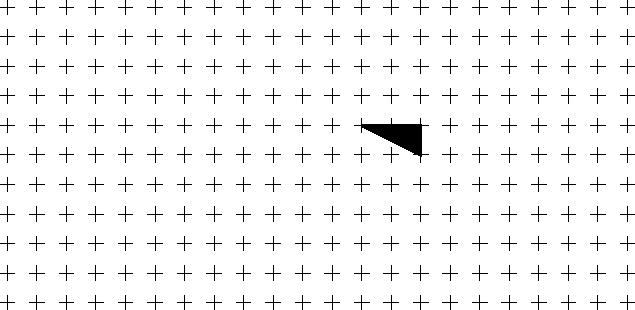
\includegraphics[width=.8\textwidth]{pinwheelInflate.pdf}
  \]
\end{enumerate}
Check with your friends to see that you get the same result.
\end{question}

\mynewpage

\begin{question}
In the pictures below, shade in (using colored pencils) the various
inflations of the shaded pinwheel triangle.
\[
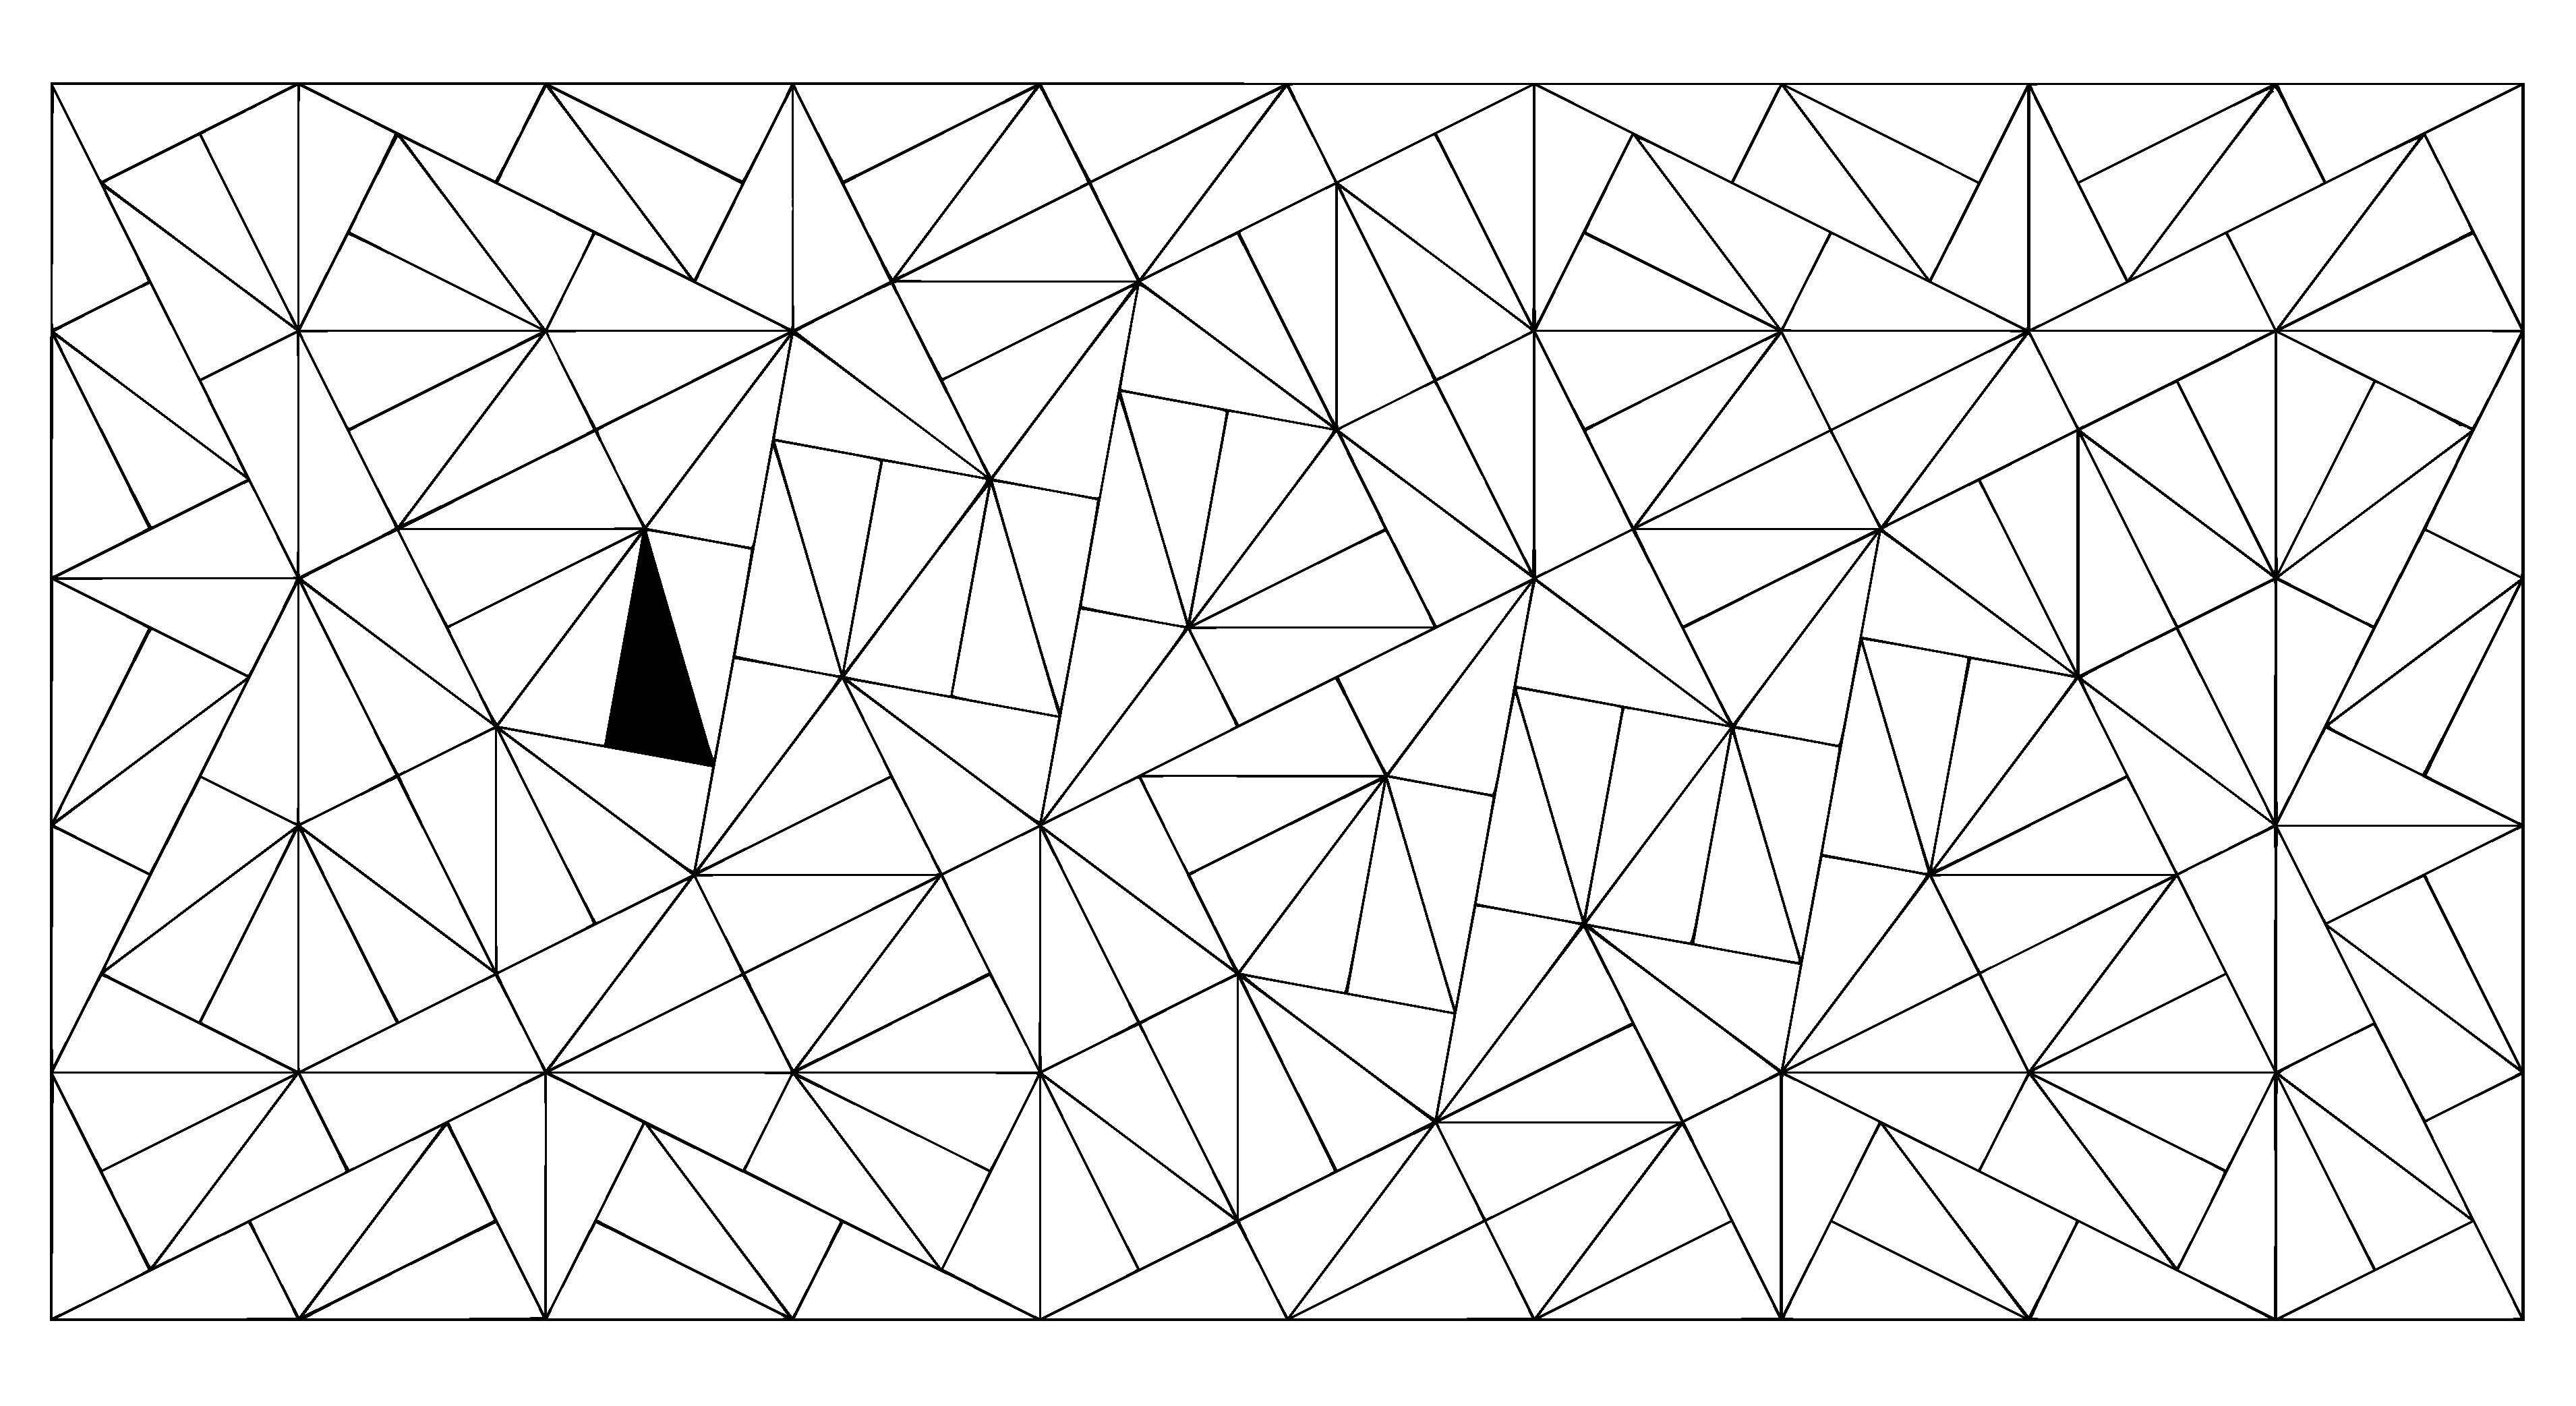
\includegraphics[width=.8\textwidth]{pinwheel1.pdf}
\]
While only the shaded triangle above is used to ``inflate'' the
pinwheel triangle, every triangle is part of \textbf{some}
inflation. In the picture below, shade in (using colored pencils) the
various inflations containing the shaded pinwheel triangle.
\[
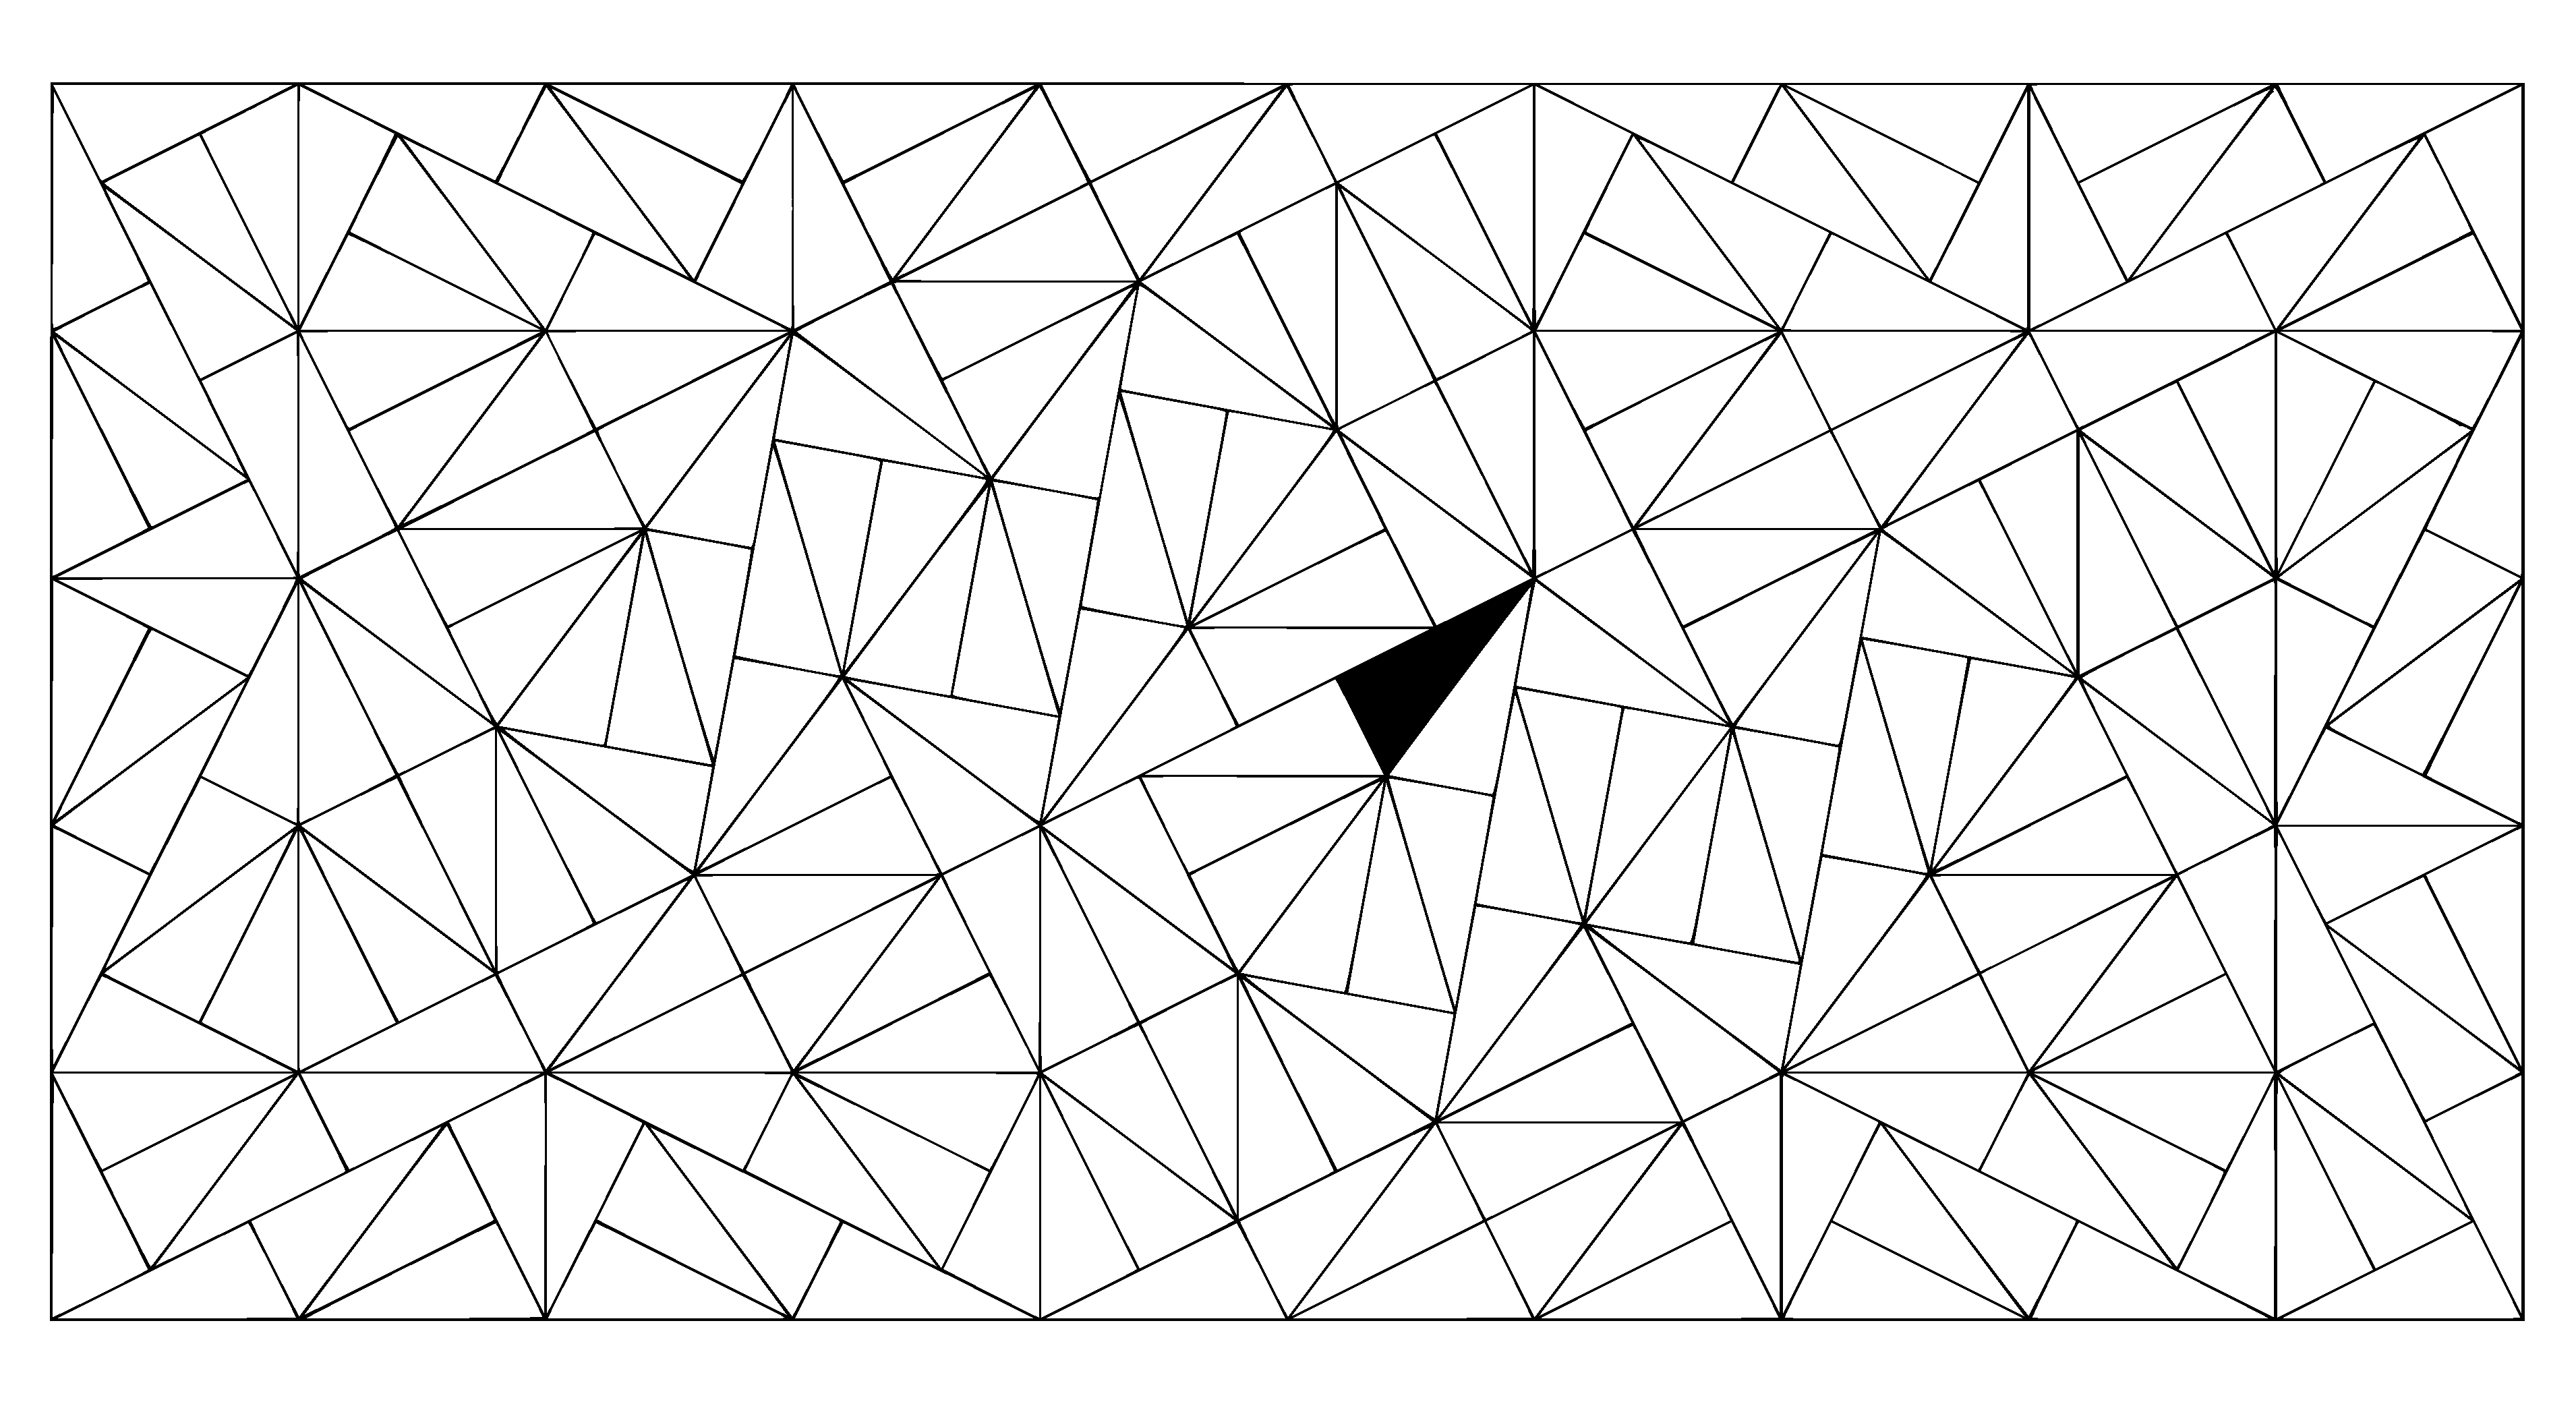
\includegraphics[width=.8\textwidth]{pinwheel2.pdf}
\]
\end{question}


\mynewpage

\begin{question}
In the picture below, shade in (using colored pencils) the
various inflations containing the shaded pinwheel triangle.
\[
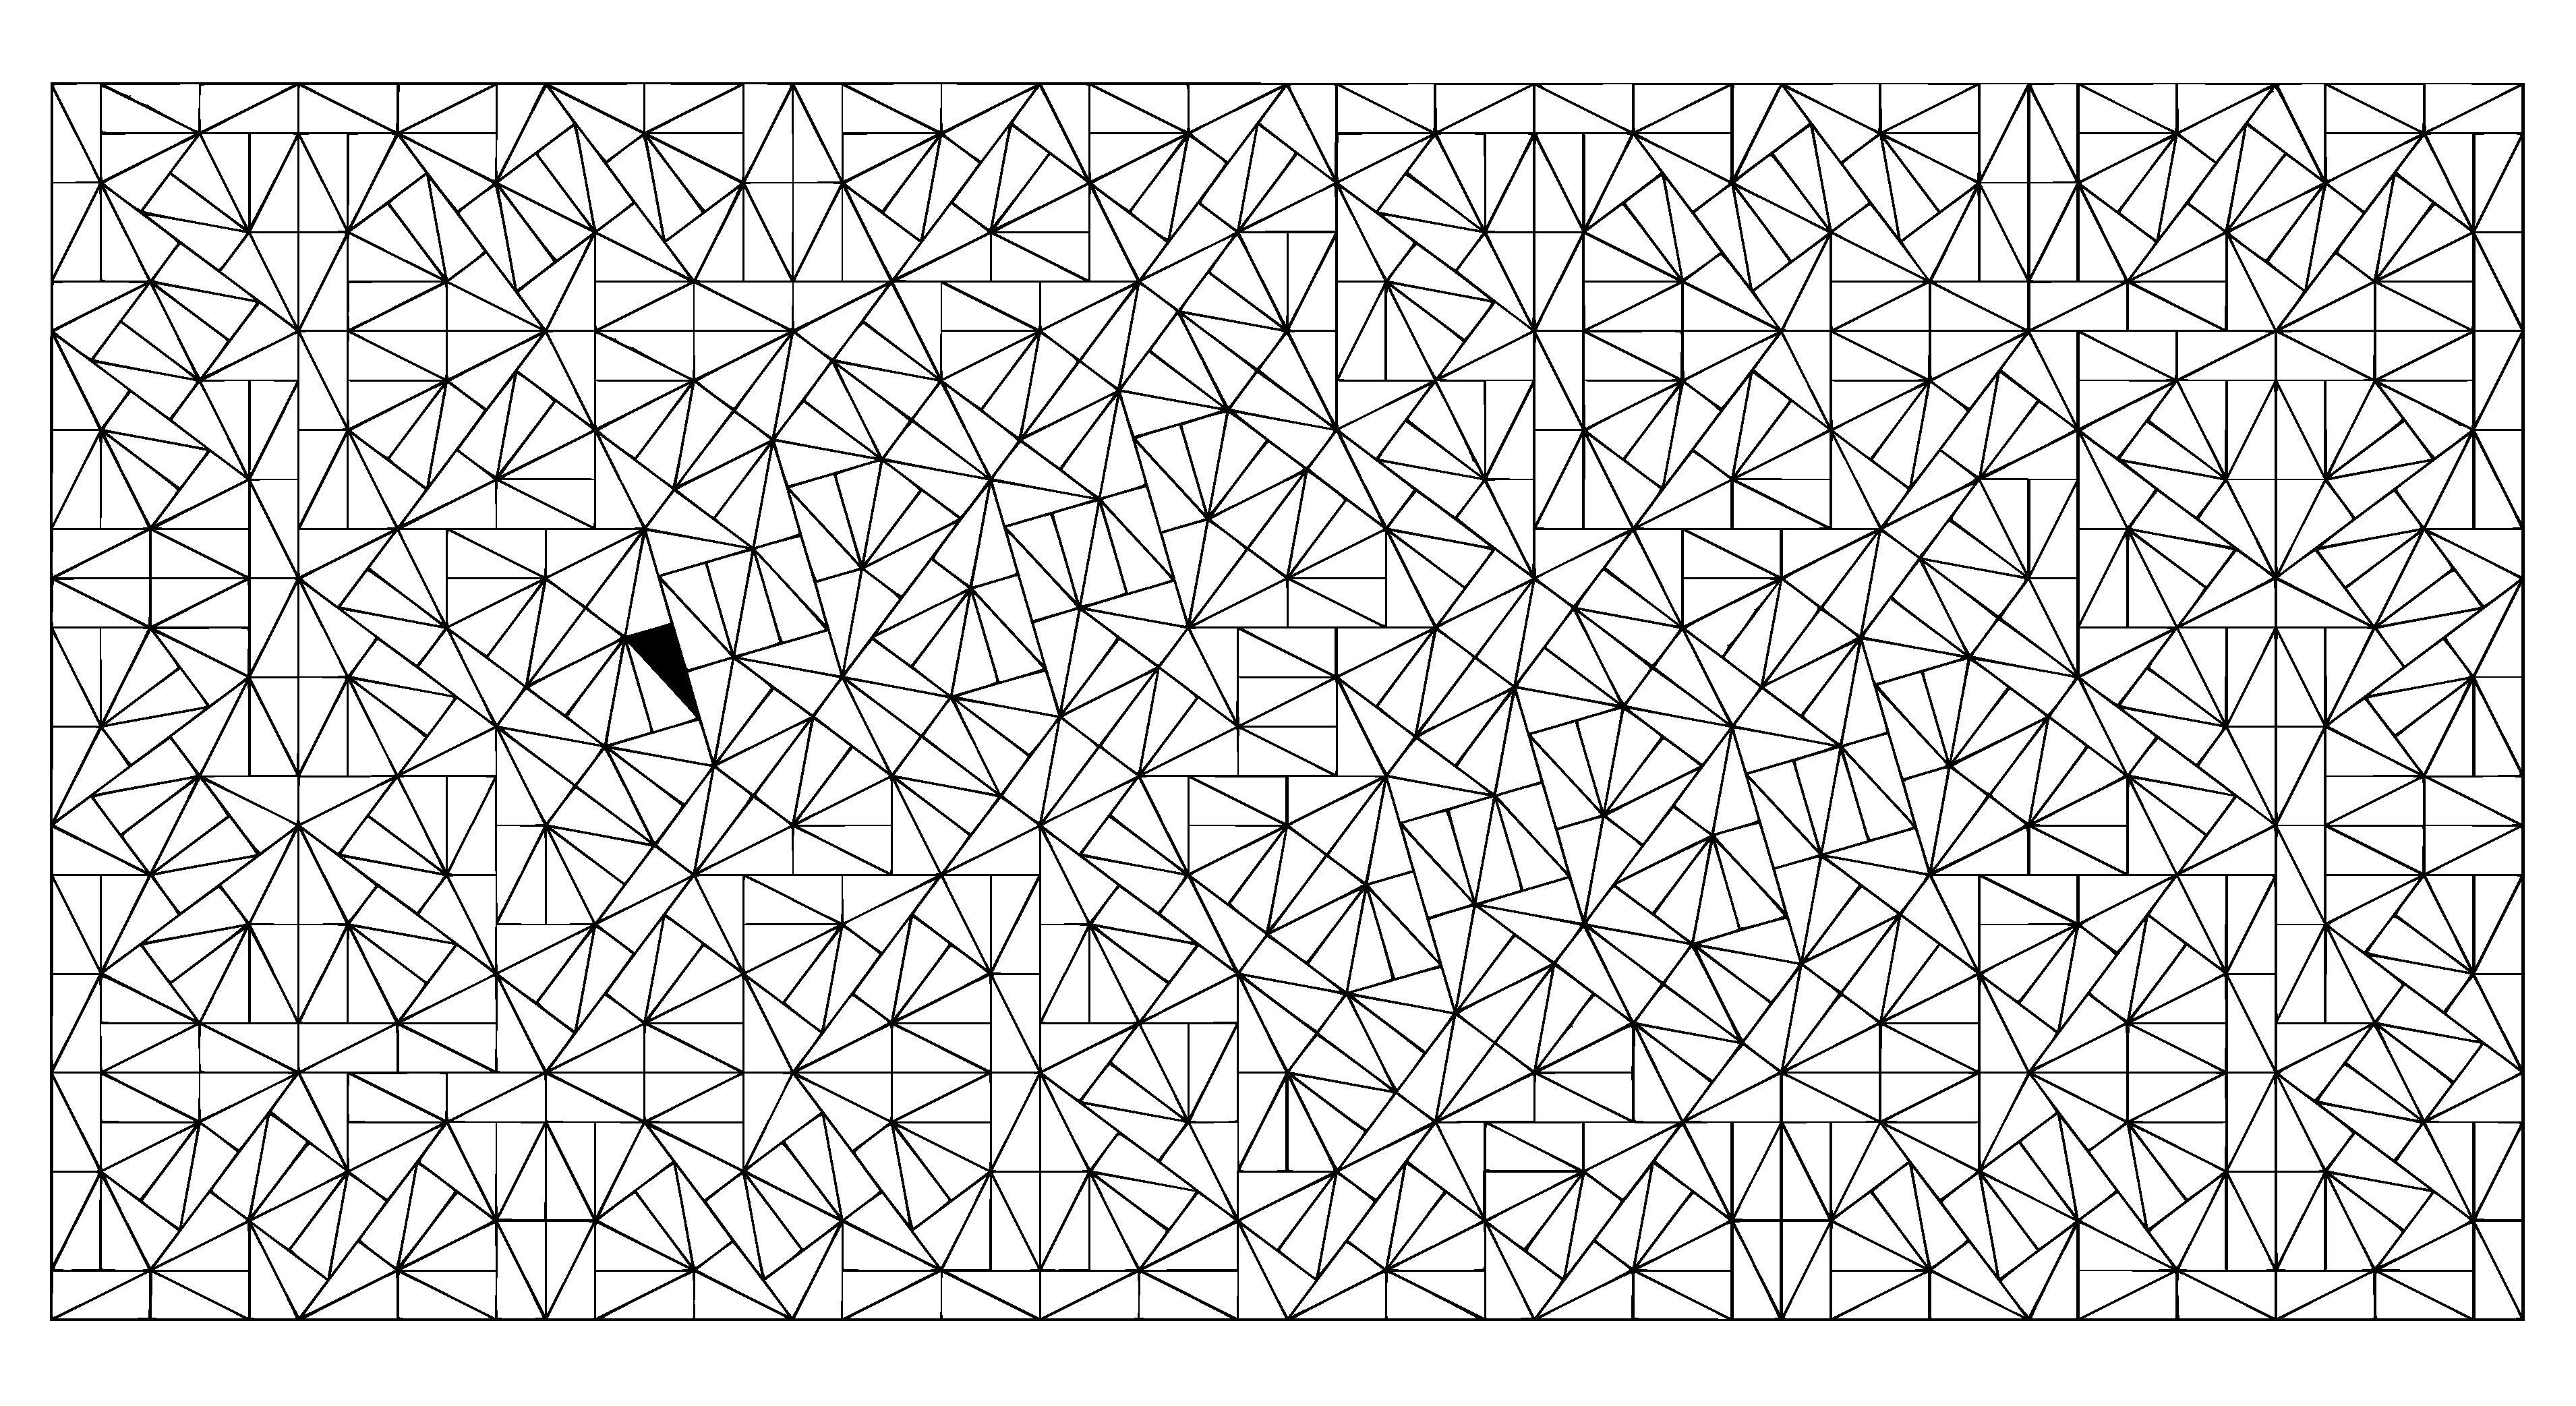
\includegraphics[width=.8\textwidth]{pinwheel3.pdf}
\]
While only the shaded triangle above is used to ``inflate'' the
pinwheel triangle, every triangle is part of \textbf{some}
inflation. In the picture below, shade in (using colored pencils) the
various inflations containing the shaded pinwheel triangle.
\[
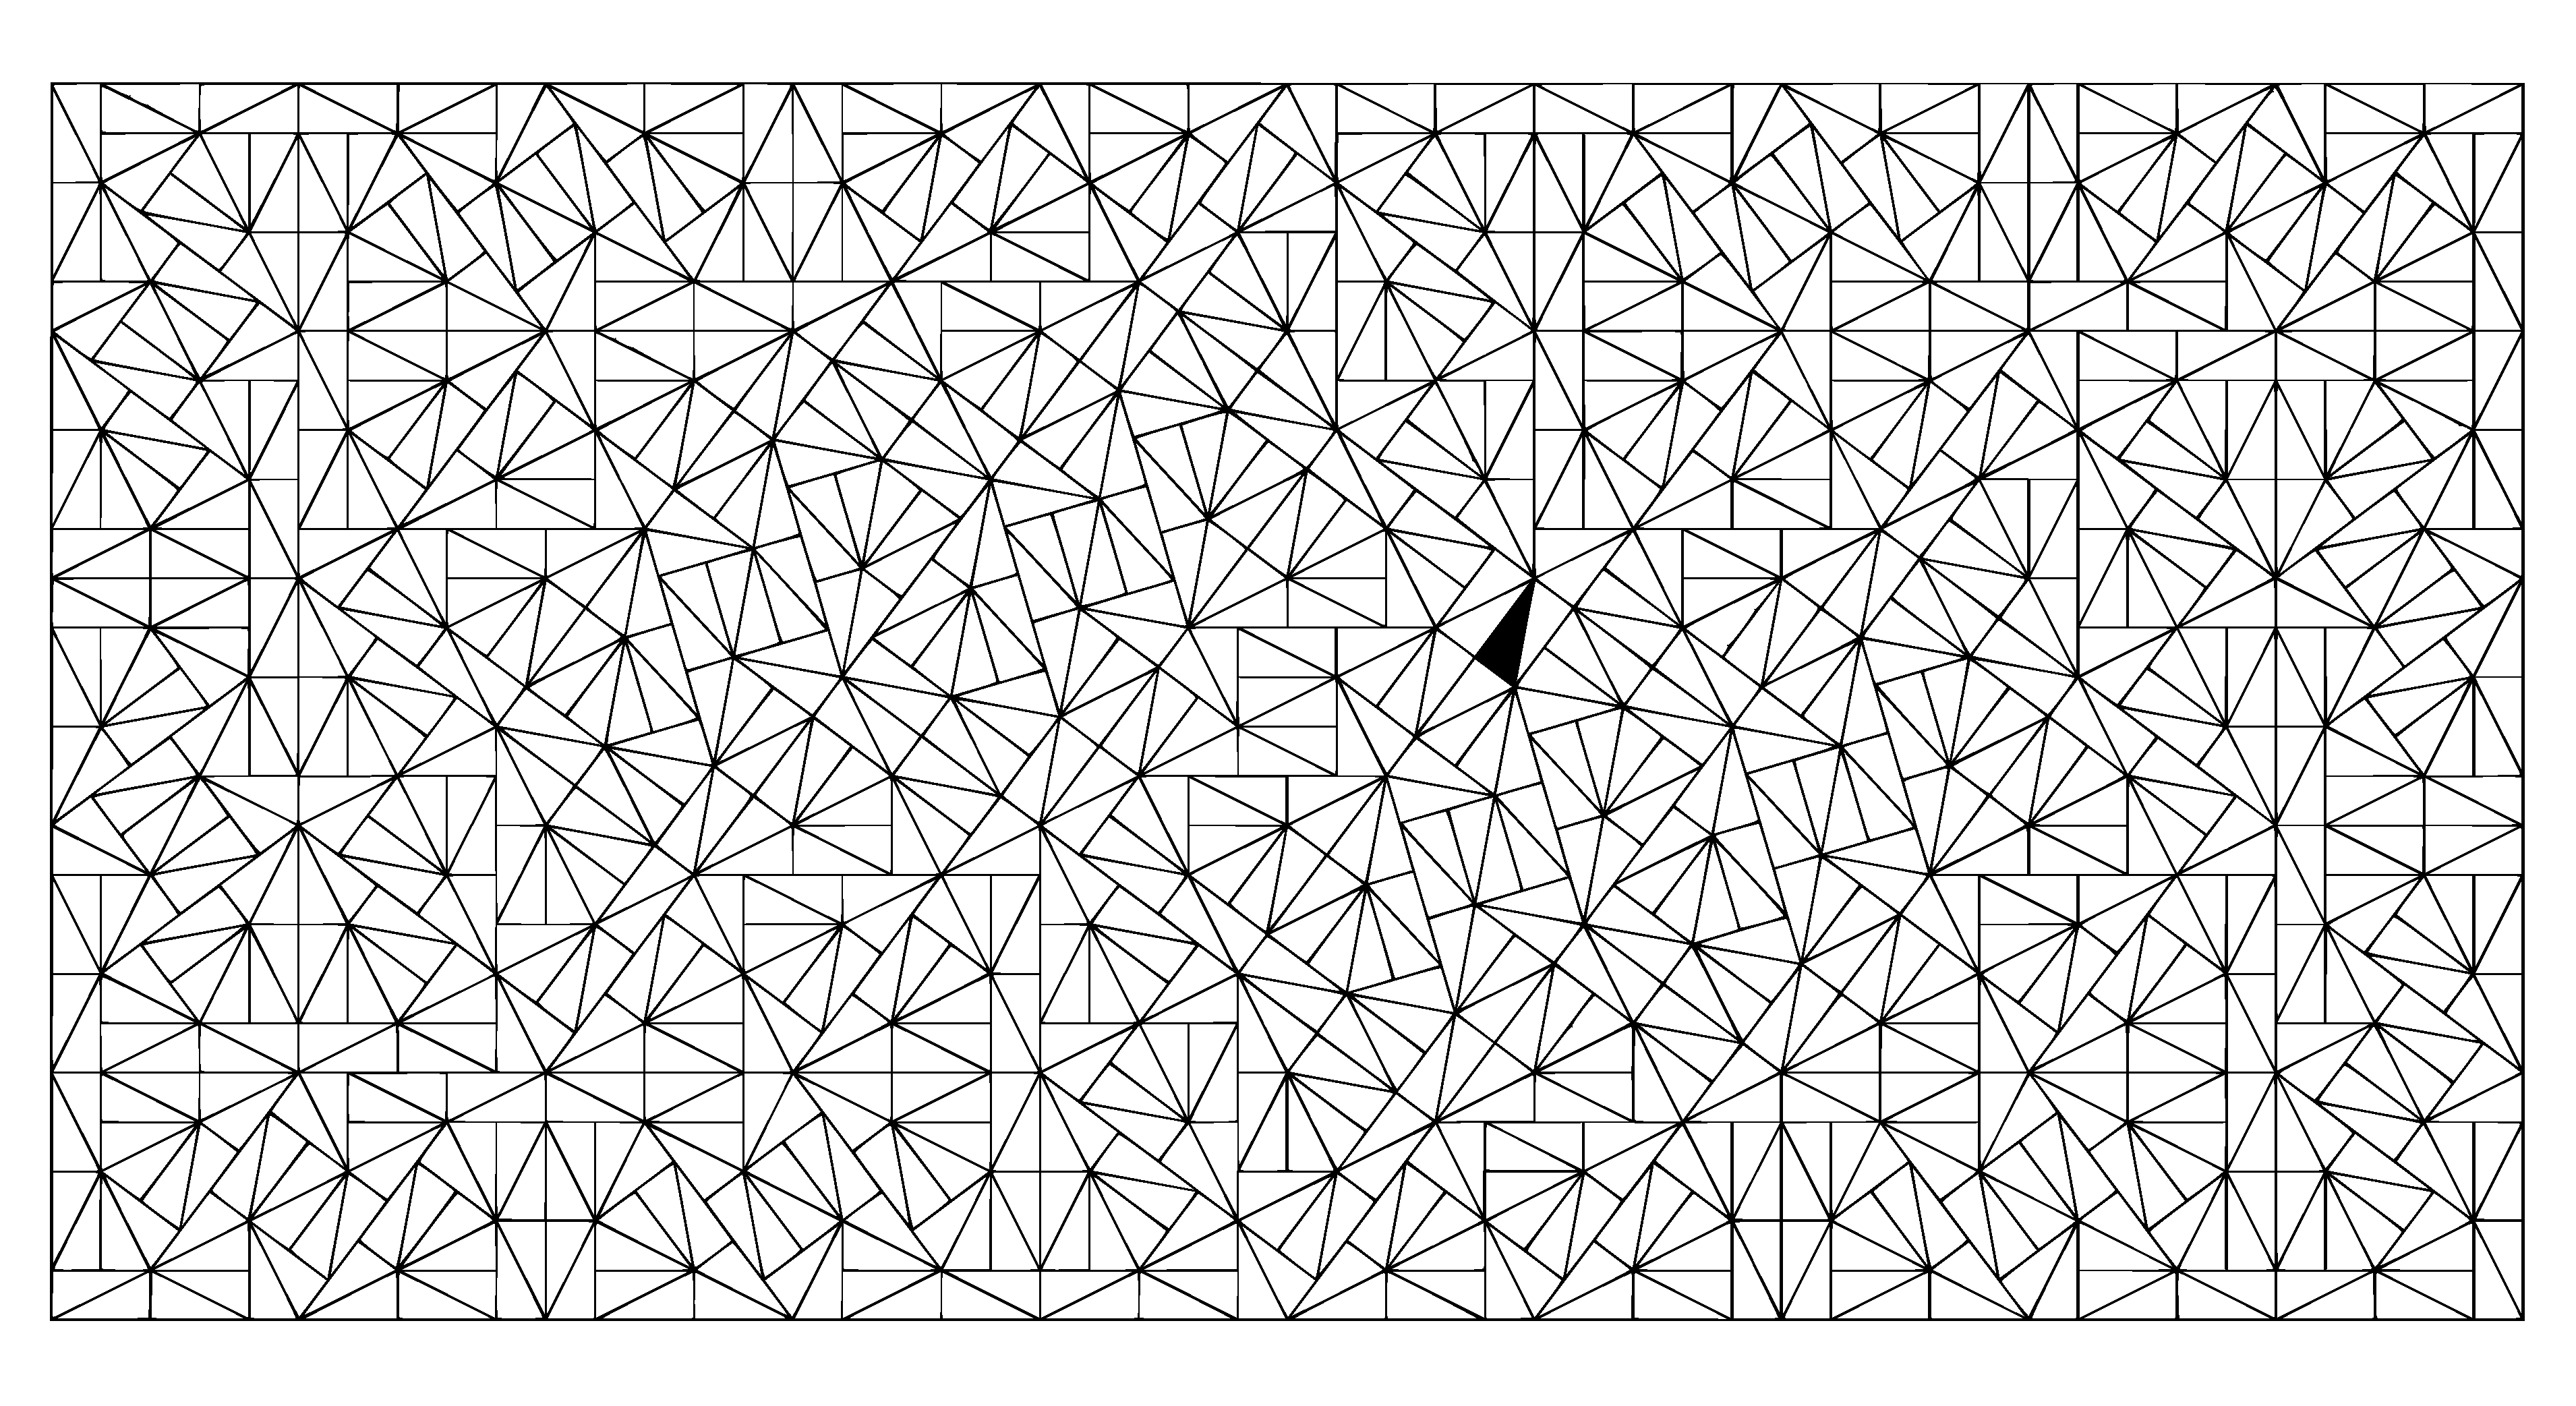
\includegraphics[width=.8\textwidth]{pinwheel4.pdf}
\]
\end{question}


%% We claim that the pinwheel tiling has no symmetry through any
%% isometry---yet it still has symmetry of scale.


%% \begin{question}
%% Explain why any triangle in a pinwheel tiling is necessarily a part of
%% one, and only one, inflation.
%% \end{question}


%% \begin{question}
%% Suppose there was an isometry that moved one triangle to another. What
%% would that say about an inflation that contained them both? Why would
%% that contradict the questionlem above?
%% \end{question}


%% \begin{question}
%% The pinwheel tiling has been used in the design of several famous
%% buildings---can you name one?
%% \end{question}


\end{document}
